
% --------------------------------------------------------------------------------------------------
% Mathematical Proof and Formal Verification
% --------------------------------------------------------------------------------------------------


\chapter{Mathematical Proof and Formal Verification}
\label{c:chapter2}

Here the next chapter \ref{c:chapter2}...
\section{Mathematical Proofs}
Given a theorem in first-order-logic one could simply enumerate proofs until a proof of the theorem is found. Of course the resources and time for such search are far from any practical relevance. \todo{how such enumeration works}.
One wishes to find a proof as quick and lean as possible and for that, different methods have been developed. We look at two such methods
\begin{enumerate}
  \item natural deduction
  \item sequent calculus
\end{enumerate}
\cite{truth_through_proof}.
Proofs can be translated from one format to another. 

\subsection{Natural Deduction}
Natural deduction is a system with rules of inference, to derive a theorem by starting from a set of axioms.\\

\subsubsection{Rules of inference}
\
\subsubsection{Sequent Calculus}


\section{Formal Verification}
Lore ipsum...

\section{Why Formalize Mathematics}
The use of Lean 4 and other proof assistants like Rocq enables mathematicians to prove propositions which are too complex and time consuming to solve 
by hand. Figure \ref{fig:model} gives a comparison. The well known \textit{4 color theorem} was not conclusively provable without formal verification. 
Large classes of counterexamples only a computer program could eliminate. This proof was controversial but verified using Rocq. \cite{web:intuitionistic_logic}

\begin{figure}[htbp]
  \centering
  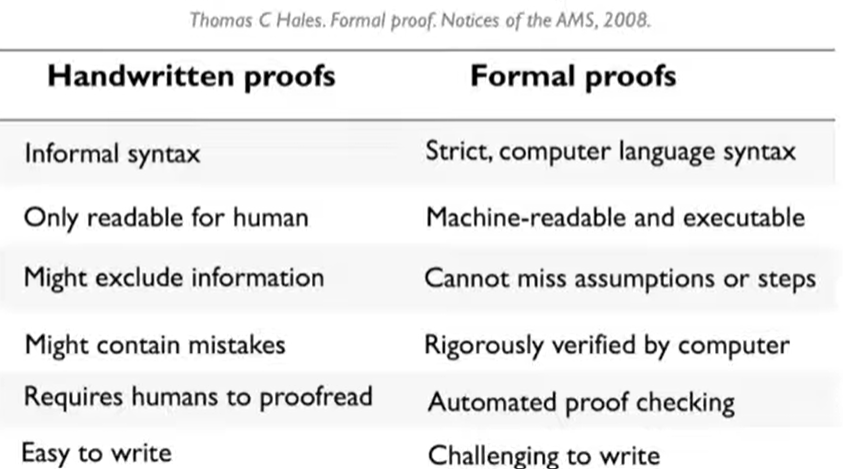
\includegraphics[width=0.7\textwidth]{figures/twokindofproofs.png}
  \caption{Ref: Lean for Scientists and Engineers, Summer 2024 - Lecture 1}
  \label{fig:model}
\end{figure}
















